\documentclass[12pt,]{article}
\usepackage{lmodern}
\usepackage{amssymb,amsmath}
\usepackage{ifxetex,ifluatex}
\usepackage{fixltx2e} % provides \textsubscript
\ifnum 0\ifxetex 1\fi\ifluatex 1\fi=0 % if pdftex
  \usepackage[T1]{fontenc}
  \usepackage[utf8]{inputenc}
\else % if luatex or xelatex
  \ifxetex
    \usepackage{mathspec}
  \else
    \usepackage{fontspec}
  \fi
  \defaultfontfeatures{Ligatures=TeX,Scale=MatchLowercase}
\fi
% use upquote if available, for straight quotes in verbatim environments
\IfFileExists{upquote.sty}{\usepackage{upquote}}{}
% use microtype if available
\IfFileExists{microtype.sty}{%
\usepackage{microtype}
\UseMicrotypeSet[protrusion]{basicmath} % disable protrusion for tt fonts
}{}
\usepackage[margin=1in]{geometry}
\usepackage{hyperref}
\hypersetup{unicode=true,
            pdftitle={2019-02-04},
            pdfauthor={Stefano Coretta},
            pdfborder={0 0 0},
            breaklinks=true}
\urlstyle{same}  % don't use monospace font for urls
\usepackage{natbib}
\bibliographystyle{unified}
\usepackage{graphicx,grffile}
\makeatletter
\def\maxwidth{\ifdim\Gin@nat@width>\linewidth\linewidth\else\Gin@nat@width\fi}
\def\maxheight{\ifdim\Gin@nat@height>\textheight\textheight\else\Gin@nat@height\fi}
\makeatother
% Scale images if necessary, so that they will not overflow the page
% margins by default, and it is still possible to overwrite the defaults
% using explicit options in \includegraphics[width, height, ...]{}
\setkeys{Gin}{width=\maxwidth,height=\maxheight,keepaspectratio}
\IfFileExists{parskip.sty}{%
\usepackage{parskip}
}{% else
\setlength{\parindent}{0pt}
\setlength{\parskip}{6pt plus 2pt minus 1pt}
}
\setlength{\emergencystretch}{3em}  % prevent overfull lines
\providecommand{\tightlist}{%
  \setlength{\itemsep}{0pt}\setlength{\parskip}{0pt}}
\setcounter{secnumdepth}{5}
% Redefines (sub)paragraphs to behave more like sections
\ifx\paragraph\undefined\else
\let\oldparagraph\paragraph
\renewcommand{\paragraph}[1]{\oldparagraph{#1}\mbox{}}
\fi
\ifx\subparagraph\undefined\else
\let\oldsubparagraph\subparagraph
\renewcommand{\subparagraph}[1]{\oldsubparagraph{#1}\mbox{}}
\fi

%%% Use protect on footnotes to avoid problems with footnotes in titles
\let\rmarkdownfootnote\footnote%
\def\footnote{\protect\rmarkdownfootnote}

%%% Change title format to be more compact
\usepackage{titling}

% Create subtitle command for use in maketitle
\newcommand{\subtitle}[1]{
  \posttitle{
    \begin{center}\large#1\end{center}
    }
}

\setlength{\droptitle}{-2em}

  \title{2019-02-04}
    \pretitle{\vspace{\droptitle}\centering\huge}
  \posttitle{\par}
    \author{Stefano Coretta}
    \preauthor{\centering\large\emph}
  \postauthor{\par}
      \predate{\centering\large\emph}
  \postdate{\par}
    \date{03/02/2019}


\begin{document}
\maketitle

\hypertarget{bayesian-meta-analysis-of-the-voicing-effect-in-english-stressed-vowels}{%
\section{Bayesian meta-analysis of the voicing effect in English
(stressed
vowels)}\label{bayesian-meta-analysis-of-the-voicing-effect-in-english-stressed-vowels}}

A Bayesian meta-analysis of the English voicing effect has been
performed on 9 studies, following the procedures in
\citet{nicenboim2018a}. The posterior distributions of each study have
been obtained by fitting a Bayesian linear model to the summary data
(means) provided in the respective papers. Only two studies,
\citet{davis1989} and \citet{ko2018}, reported measures of dispersion
along with measures of central tendency. A measurement error model was
used to obtain the posterior distributions from these studies. In two
cases, \citet{sharf1962} and \citet{klatt1973}, the authors tested both
monosyllabic and disyllabic words, so two separate distributions were
calculated for each word type. This leads to a total of 11 posterior
distribution of the effect of consonant voicing on vowel duration in
English. A data set with the mean estimates and estimated standard
errors from this 11 posterior distributions has been used to fit a
Bayesian error model, which had the mean estimate as outcome, and the
intercept and a by-study random intercept as predictors.

The effect estimated by the meta-analysis (the intercept of the mean
estimate) is +58.28 ms (Est. error = 12.99) when C2 is voiced, with the
95\% credible intervals (CI) between 33.31 and 84.63. The following plot
shows the posterior distribution of the estimated voicing effect. The
darker area represents the 50\% CI, while the dark think line is the
median.

\begin{center}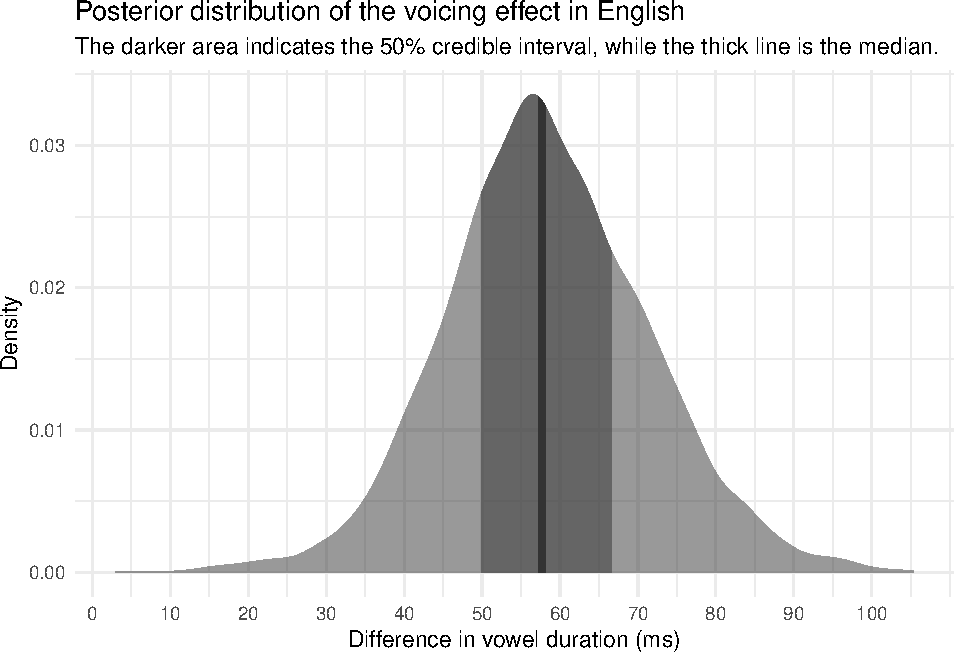
\includegraphics[width=5in,height=3.5in]{2019-02-04_files/figure-latex/ve-est-post-1} \end{center}

In the following funnel plot, the mean estimate (the points) of the
voicing effect with 95\% CIs (the horizontal segments) is shown for each
of the 11 studies. For each study, the plot gives both the original
estimate (as obtained from the original data summary of the study) and
the estimate calculated by the random effects in the meta-analytical
model. The vertical lines indicate the meta-analytical mean estimate
(the thick line) and the 95\% CI (the dashed lines). Note how the
studies in which the target vowel was in a non-final syllable have a
smaller estimate.

\begin{center}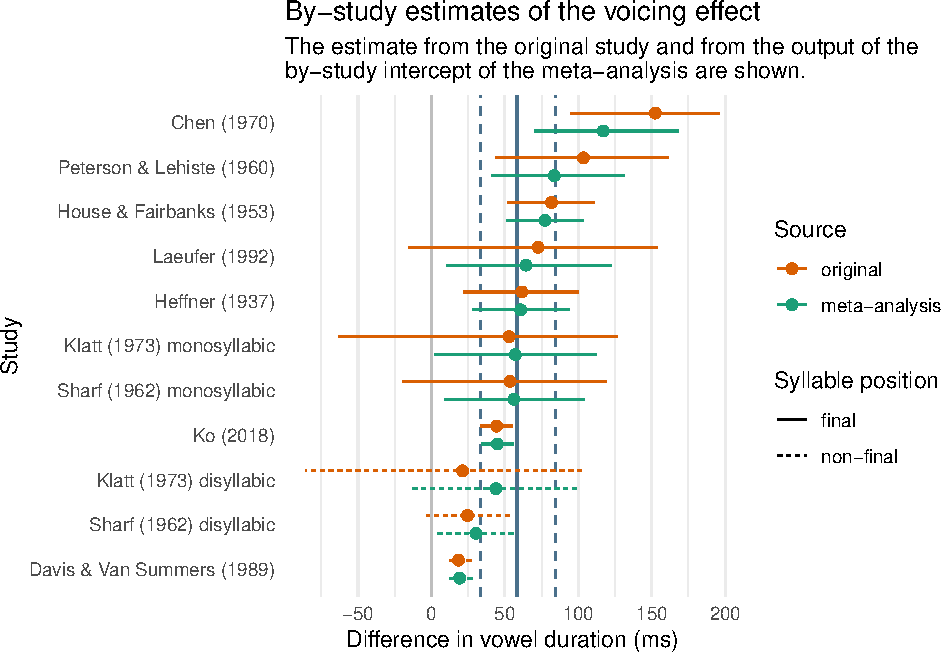
\includegraphics[width=6in,height=4.5in]{2019-02-04_files/figure-latex/origin-shrunk-1} \end{center}

In a follow-up analysis, the within-word position of the syllable with
the test vowel has been included as a predictor. The following figure
shows the posterior distributions of the voicing effect in word final
and non-final syllables respectively. According to the meta-analytical
model, the effect of voicing is +70.69 ms (SE = 12.36, 95\% CI =
47.03:95.61) in word-final syllables, and +25.46 (\(\hat{\beta{}}\) =
-45.23, SE = 19.50, 95\% CI = -84.36:-5.38) in non-final syllables.

\begin{center}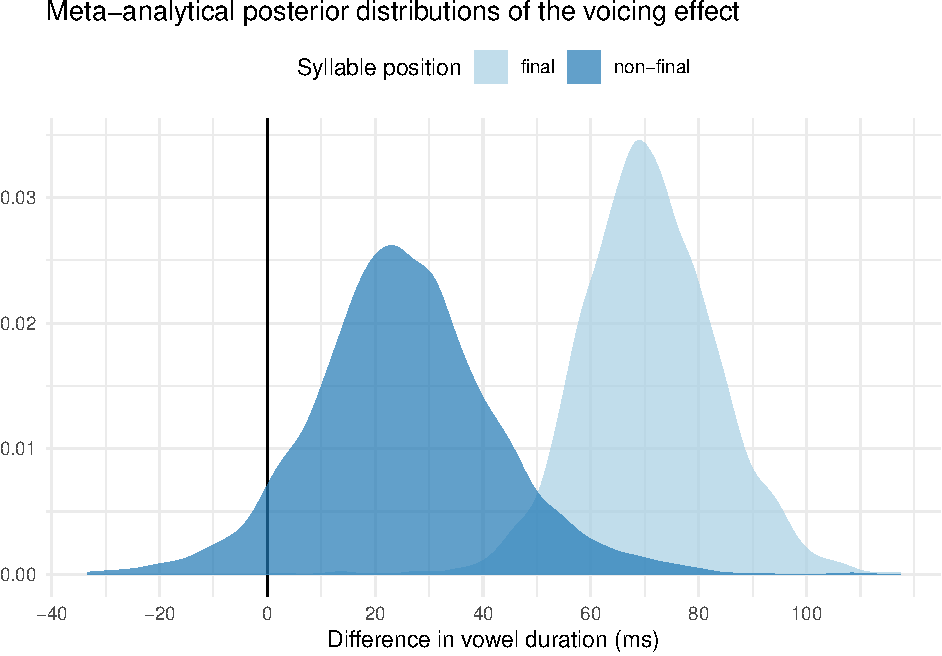
\includegraphics[width=5in,height=3.5in]{2019-02-04_files/figure-latex/syl-plot-1} \end{center}

\nocite{chen1970, peterson1960, house1953, laeufer1992, heffner1937, klatt1973, sharf1962, ko2018, davis1989}

\bibliography{linguistics}


\end{document}
